\documentclass[aspectratio=169, 14pt]{beamer}
\usepackage{scalefnt}
\usepackage[utf8]{inputenc}
\usepackage[english]{babel}
\usepackage{tipa}
\usepackage{graphicx}
\usepackage{transparent}
\usepackage[ruled, lined, linesnumbered, commentsnumbered]{algorithm2e}
\usepackage{pgfplots}
\newcommand\mycommfont[1]{\small\ttfamily\textcolor{blue}{#1}}
\SetCommentSty{mycommfont}
\renewcommand{\thealgocf}{}
\usepackage{setspace}
\usepackage{tikz}
\usetikzlibrary{matrix,backgrounds}
\usetikzlibrary{arrows}
\usetikzlibrary {arrows.meta}
\usetikzlibrary{calc,shadows.blur,fit,positioning}
\usetikzlibrary{shapes.multipart,chains}
\usetikzlibrary{shadows,patterns,shapes}
\usepackage{minted}
\usepackage{fontawesome5}
\usepackage{booktabs}
\usepackage{caption}
\usepackage{hyperref}
\hypersetup{
    colorlinks=true,
    linkcolor=blue,
    filecolor=magenta,      
    urlcolor=cyan,
    }
\urlstyle{same}
\usetheme{metropolis}
\metroset{block=fill}
\usecolortheme{default}
\definecolor{darkmidnightblue}{rgb}{0.0, 0.2, 0.4}
\definecolor{LightGray}{gray}{0.9}

\usepackage{xparse}

\ExplSyntaxOn
\NewDocumentCommand{\DefineDictionary}{mm}
 {
  \arclupus_dict_def:nn { #1 } { #2 }
 }

\seq_new:N \l__arclupus_dict_temp_seq

\cs_new_protected:Nn \arclupus_dict_def:nn
 {
  \prop_gclear_new:c { g_arclupus_#1_dict_prop }
  \clist_map_inline:nn { #2 }
   {
    \__arclupus_dict_add:nn { #1 } { ##1 }
   }
  \cs_new:cpn { #1 } ##1 { \prop_item:cn { g_arclupus_#1_dict_prop } { ##1 } }
 }

\cs_new_protected:Nn \__arclupus_dict_add:nn
 {
  \seq_set_split:Nnn \l__arclupus_dict_temp_seq { / } { #2 }
  \prop_gput:cxx { g_arclupus_#1_dict_prop }
   {
    \seq_item:Nn \l__arclupus_dict_temp_seq { 1 }
   }
   {
    \seq_item:Nn \l__arclupus_dict_temp_seq { 2 }
   }
 }
\cs_generate_variant:Nn \prop_gput:Nnn { cxx }
\ExplSyntaxOff

\DefineDictionary{var}{1/A, 2/B, 3/C}

% The logic for Hanoi, we record the discs at every pole
% as a comma separated list ending with a '.'; i.e. the
% starting list for 4 discs would be 1,2,3,4,.
\newcount\ndiscs
\def\initpoles#1{
    \def\disclist{}
    \foreach \n in {1,...,#1} {
        \xdef\disclist{\disclist\n,}
    }
    \expandafter\xdef\csname pole 1\endcsname{\disclist.}
    \expandafter\gdef\csname pole 2\endcsname{.}
    \expandafter\gdef\csname pole 3\endcsname{.}
}

% Delimited macro; #1 is everything up to the first ',' and
% #2 everything after it.
\def\head#1,#2.{#1}
\def\tail#1,#2.{#2}

% This macro updates the disc lists, its arguments are the name
% names of the macro's corresponding to the poles, for example
% 'pole 1' and 'pole 3'.
\def\movedisc#1#2{
    \edef\lista{\csname #1\endcsname}
    \edef\listb{\csname #2\endcsname}
    \expandafter\xdef\csname #2\endcsname{\expandafter\head\lista,\listb}
    \expandafter\xdef\csname #1\endcsname{\expandafter\tail\lista.}
}

% Updates the lists and then draws a new frame.
\def\move#1#2{
    \movedisc{pole #1}{pole #2}
    \gdef\fmsg{\node[anchor=north] at (3.8,-.5) {Moved disc from pole \var{#1} to pole \var{#2}.};}
    \drawpoles
}

% This macro boils down to a well-known recursive solution, as given
% here for example: http://en.wikipedia.org/wiki/Towers_of_Hanoi#Recursive_solution
%
% #1 Pole to move from
% #2 Pole to move to
% #3 Pole to use as scratch
% #4 Number of disks
\def\rhanoi#1#2#3#4{
    \ifnum#4>1
        {\advance#4 by -1 \rhanoi#1#3#2#4}
        \move{#1}{#3}
        {\advance#4 by -1 \rhanoi#2#1#3#4}
    \else
        \move{#1}{#3}
    \fi
}

% Below is the TikZ code to draw the towers:
\tikzset{
    disc/.style={shade, shading=radial, rounded rectangle,minimum height=.5cm,
        inner color=#1!20, outer color=#1!60!gray},
    disc 1/.style={disc=yellow, minimum width=15mm},
    disc 2/.style={disc=orange, minimum width=20mm},
    disc 3/.style={disc=red, minimum width=25mm},
    disc 4/.style={disc=green, minimum width=30mm},
    disc 5/.style={disc=blue, minimum width=35mm},
    disc 6/.style={disc=purple, minimum width=40mm},
}

% Define some colors, I don't like plain green and brown.
\definecolor{darkgreen}{rgb}{0.2,0.55,0}
\definecolor{darkbrown}{rgb}{0.375,0.25,0.125}

\newcommand{\pole}{
  \fill[darkbrown] (-1.6cm, 0) rectangle (1.6cm,0.25cm)
    (-1.25mm,2.5mm) rectangle (1.25mm,4.25cm);
}

% Because the list starts with the topmost disc, we
% use two recursive macro's to invert the drawing process.
\newcount\curlevel

% This macro checks whether the list is empty, if not,
% it calls \rdrawdiscs which removes one element and
% calls this one again.

\def\drawdiscs#1.{
    % If #1 is empty, this expands to \if.. which is true, otherwise
    % we're safe to assume there's at least one element.
    \expandafter\if#1..\else
        \rdrawdiscs#1.
        \advance\curlevel by 1\relax
    \fi
}

\def\rdrawdiscs#1,#2.{
    \drawdiscs#2.
    {\edef\n{\the\curlevel}
        % Draw the actual disk.
        \node[disc #1,yshift={\n*5mm}] {#1};
    }
}

\def\discs#1{
    \curlevel=1
    \expandafter\drawdiscs#1
}

% Draws the whole situation based on the lists.
\def\drawpoles{
    \begin{frame}{\ftitle}
    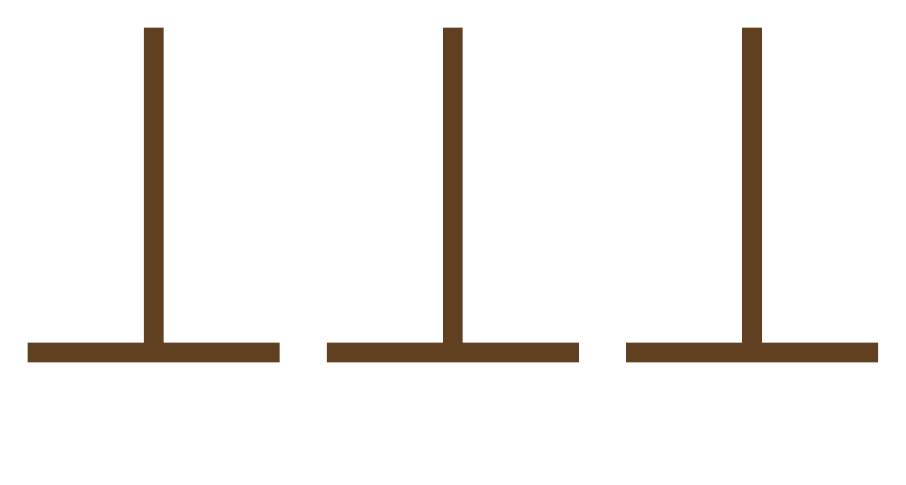
\begin{tikzpicture}
        \foreach \n/\x in {1/0cm,2/3.8cm,3/7.6cm} {
            \begin{scope}[xshift=\x]
                \pole
                \expandafter\discs\csname pole \n\endcsname
            \end{scope}
        }
        % Macro that either contains something like OK or
        % the last move.
        \fmsg
        % We use this to prevent the picture from jumping between
        % frames.
        \useasboundingbox (-1.6cm,-1.2cm) rectangle (9.2cm,4.25cm);
    \end{tikzpicture}
    \end{frame}
}
\def\hanoi#1{
    \ndiscs=#1
    \initpoles{#1}
    \xdef\ftitle{Towers of Hanoi}
    \gdef\fmsg{}
    % Starting frame.
    \drawpoles
    % Recursion draws a new frame for every step.
    \rhanoi{1}{2}{3}{\ndiscs}
    % Final frame.
    \gdef\fmsg{\node[] at (3.8,2.5) {\Huge\scalefont{2}\color{darkgreen}OK};}
    \drawpoles
}
% Main macro, inits the lists for the current number, sets a title
% for the frame and starts the recursion.

%------------------------------------------------------------
%This block of code defines the information to appear in the
%Title page
\title[Data Structures] %optional
{Data Structures}

\subtitle{Lab}

\author[CHEN Zhongpu] % (optional)
{CHEN Zhongpu}

\institute[] % (optional)
{
  School of Computing and Artificial Intelligence \\
  \href{mailto:zpchen@swufe.edu.cn}{zpchen@swufe.edu.cn}
}

\date[] % (optional)
{SWUFE, Fall 2022}

%End of title page configuration block
%------------------------------------------------------------


%------------------------------------------------------------
%The next block of commands puts the table of contents at the 
%beginning of each section and highlights the current section:

% \AtBeginSection[]
% {
%   \begin{frame}
%     \frametitle{Table of Contents}
%     \tableofcontents[currentsection]
%   \end{frame}
% }
%------------------------------------------------------------


\begin{document}

%The next statement creates the title page.
\frame{\titlepage}

%---------------------------------------------------------
%This block of code is for the table of contents after
%the title page
% \begin{frame}
% \frametitle{Table of Contents}
% \tableofcontents
% \end{frame}
%--------------------------------------------------------
\begin{frame}
    \frametitle{Review}
    \begin{enumerate}
        \item Stack
        \item Queue (deque)
        \item Linked list
    \end{enumerate}
\end{frame}

{
    % \usebackgroundtemplate{\transparent{0.3}{\begin{picture}
    %     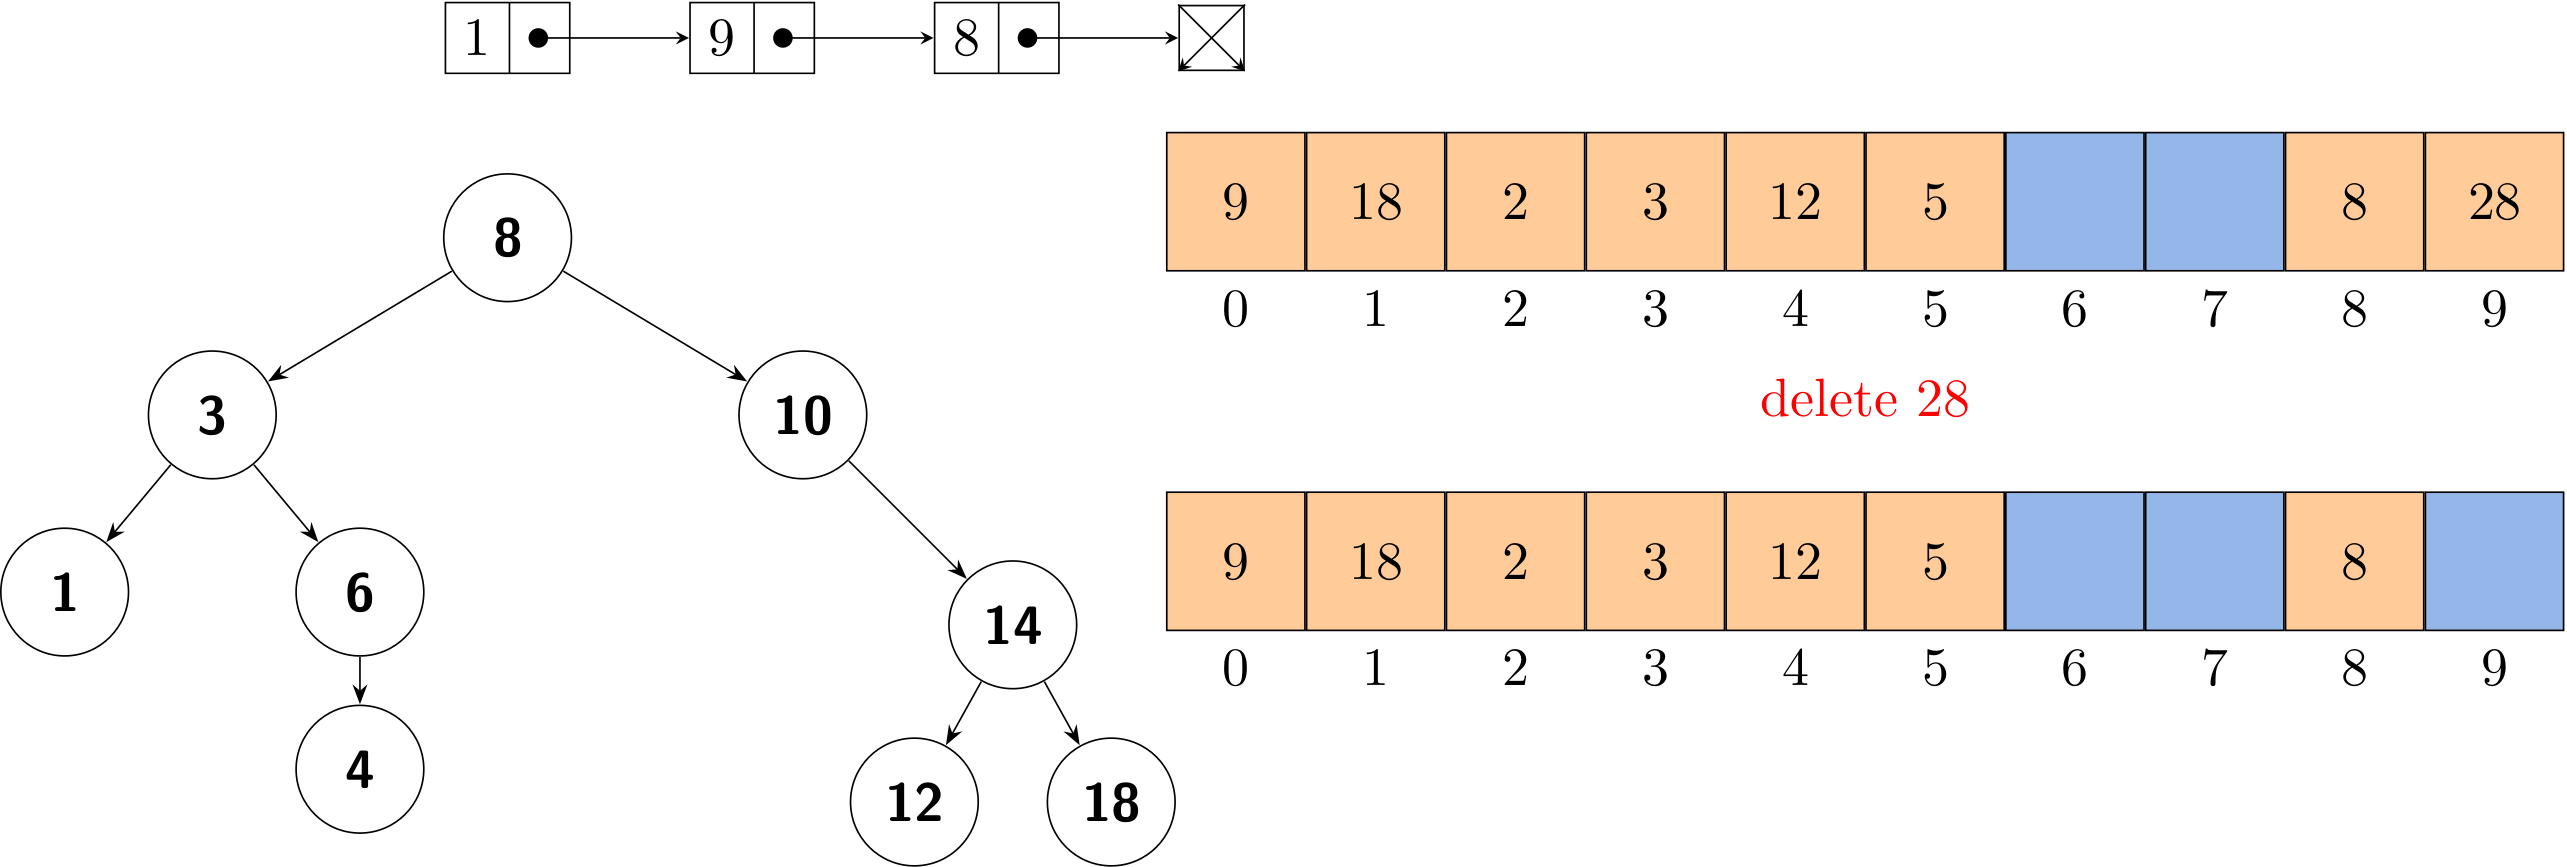
\includegraphics[height=0.7\paperheight]{cover}
    % \end{picture}    
    % }}
\usebackgroundtemplate{
  \tikz[overlay,remember picture] 
  \node[opacity=0.3, at=(current page.south east),anchor=south east, yshift=2cm,xshift=4cm] {
    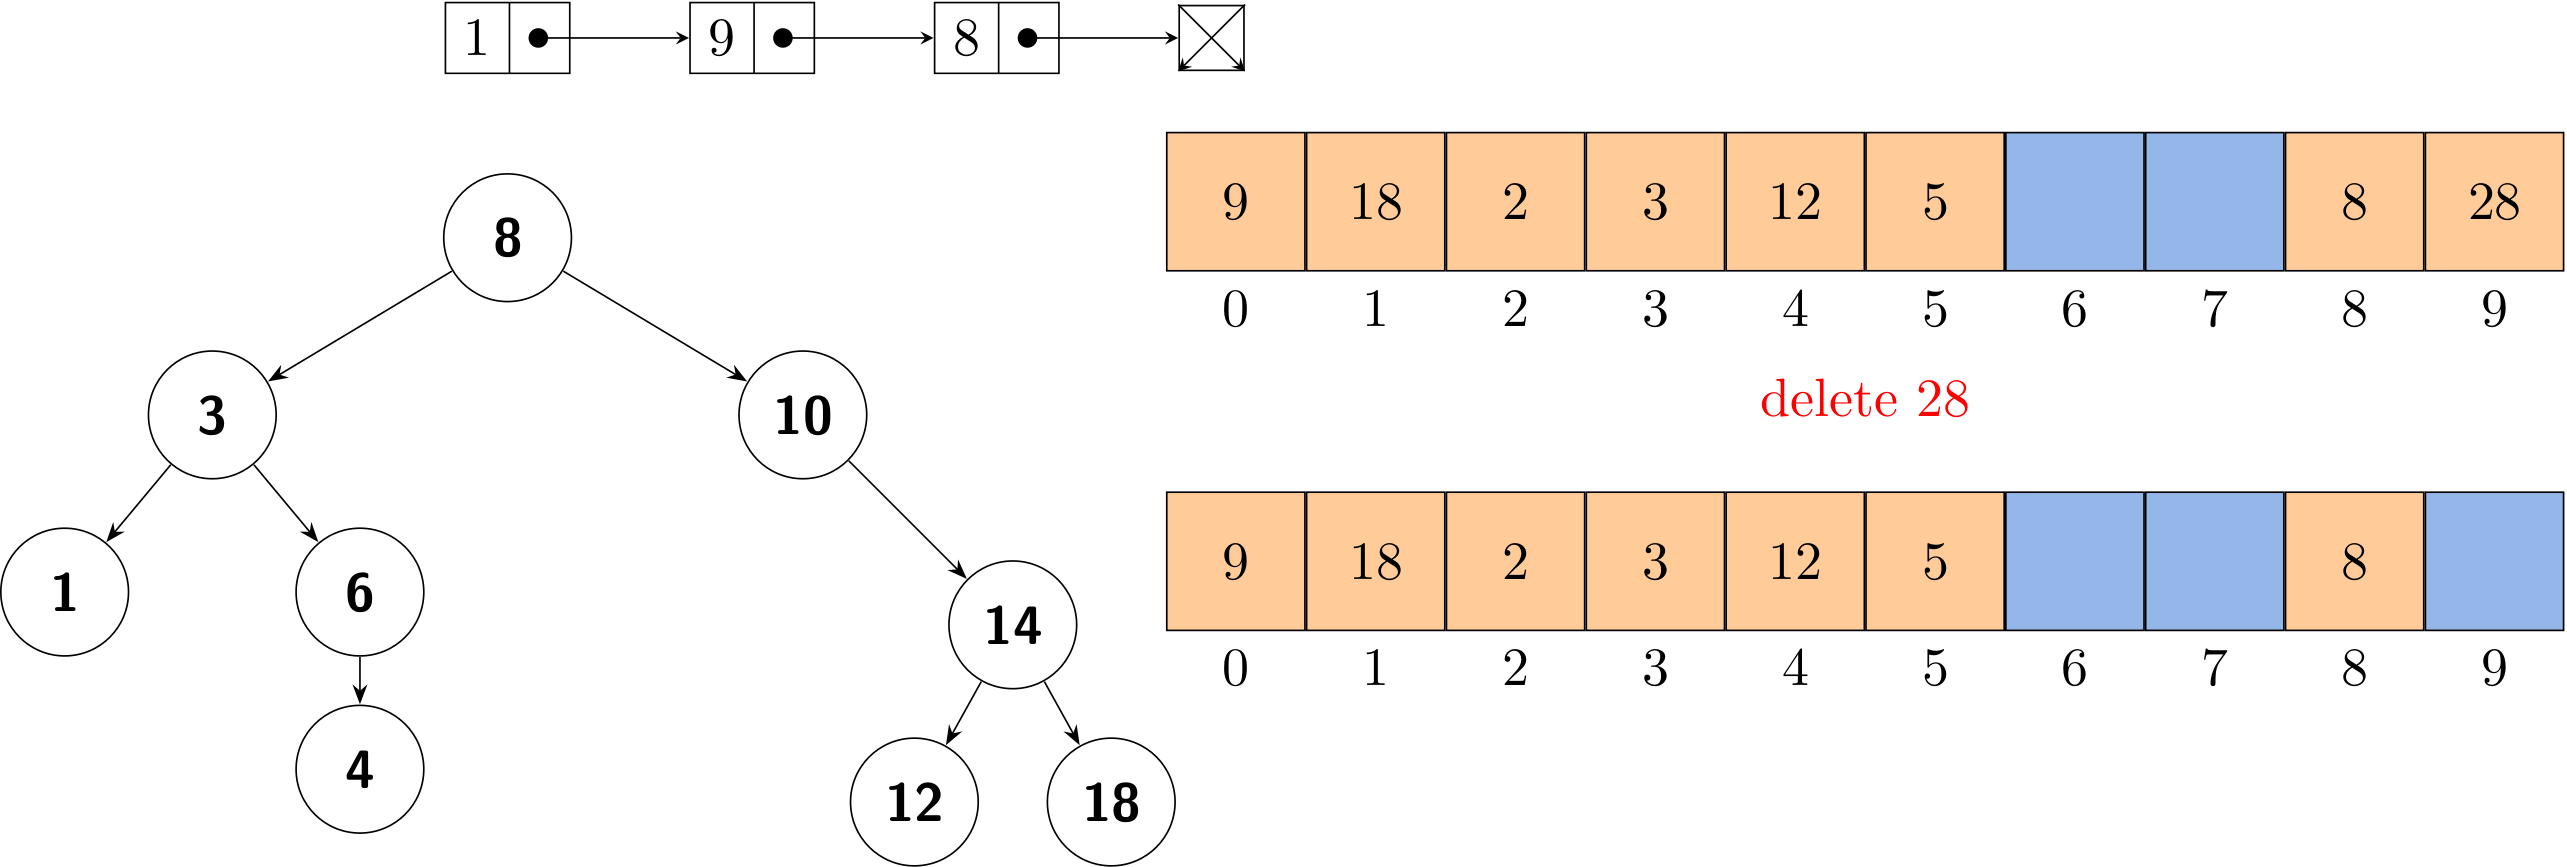
\includegraphics[height=0.6\paperheight]{cover}};
}
    \begin{frame}
        \section{\textcolor{darkmidnightblue}{1. Lab}}
    \end{frame}

}


\begin{frame}

    \section{\textcolor{darkmidnightblue}{2. Recursion}} 

    \begin{quote}
        Recursion (adjective: recursive) occurs when a thing is defined in terms of itself or of its type.
    \end{quote}

\end{frame}

\begin{frame}[fragile]
    \frametitle{2.1 Example}

\begin{columns}
    \column{.5\textwidth}<1->
    The \textbf{Fibonacci} sequence:
\begin{itemize}
    \item $F(0) = 0$
    \item $F(1) = 1$
    \item $F(2) = 1$
    \item $F(n) = F(n - 1) + F(n - 2)$
\end{itemize}
    \column{.5\textwidth}<2->
    The \textbf{Linked list}:

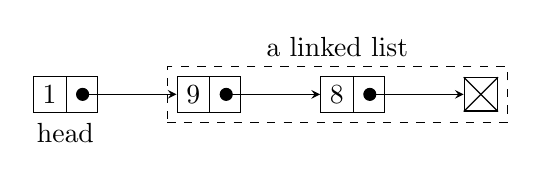
\begin{tikzpicture}[list/.style={rectangle split, rectangle split parts=2,
    draw, rectangle split horizontal}, >=stealth, start chain]

  \node[list,on chain] (A) {1};
  \node[list,on chain] (B) {9};
  \node[list,on chain] (C) {8};
  \node[on chain,draw,inner sep=6pt] (D) {};
  \draw (D.north east) -- (D.south west);
  \draw (D.north west) -- (D.south east);
  \draw[*->] let \p1 = (A.two), \p2 = (A.center) in (\x1,\y2) -- (B);
  \draw[*->] let \p1 = (B.two), \p2 = (B.center) in (\x1,\y2) -- (C);
  \draw[*->] let \p1 = (C.two), \p2 = (C.center) in (\x1,\y2) -- (D);
  \node[below=of A, yshift=1cm] (head){\alert{head}};

  \node[fit=(B)(C)(D), dashed, draw](remain) {};

  \node[above=of remain, yshift=-1cm]{\alert{a linked list}};

\end{tikzpicture}
\end{columns}

\end{frame}

\begin{frame}[fragile]
    \frametitle{2.2 Recursive Algorithm}

    \begin{itemize}
        \item Base step
        \item Recursive step
    \end{itemize}
    
    \begin{minted}[bgcolor=LightGray]{python}
def fibonacci(n):
    if n == 0:
        return 0
    elif n == 1 or n == 2:
        return 1
    else:
        return fibonacci(n - 1) + fibonacci(n - 2)        
    \end{minted}
\end{frame}

\begin{frame}[fragile]
 Get the length of a list recursively:
 \begin{equation*}
    \begin{split}
    length([1, 9, 8]) & = 1 + length([9, 8]) \\
     & = 1 + 1 + length([9]) \\
     & = 1 + 1 + 1 + length([]) \\
     & = 1 + 1 + 1 + 0
    \end{split}
\end{equation*}

    \begin{minted}[bgcolor=LightGray]{python}
def len_of_list(a):
    if len(a) == 0:
        return 0
    return 1 + len_of_list(a[1:])
\end{minted}

\end{frame}

\begin{frame}
    \frametitle{Exercise}
\begin{columns}
    \column{.5\textwidth}
    {\large \faIcon{code}} Given a linked list with \alert{head}, how to get its length recursively?
    \column{.5\textwidth}
    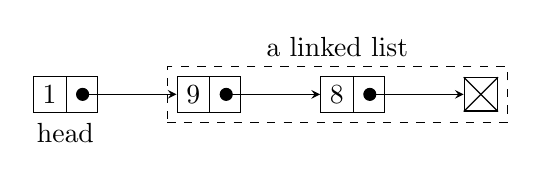
\begin{tikzpicture}[list/.style={rectangle split, rectangle split parts=2,
        draw, rectangle split horizontal}, >=stealth, start chain]
    
      \node[list,on chain] (A) {1};
      \node[list,on chain] (B) {9};
      \node[list,on chain] (C) {8};
      \node[on chain,draw,inner sep=6pt] (D) {};
      \draw (D.north east) -- (D.south west);
      \draw (D.north west) -- (D.south east);
      \draw[*->] let \p1 = (A.two), \p2 = (A.center) in (\x1,\y2) -- (B);
      \draw[*->] let \p1 = (B.two), \p2 = (B.center) in (\x1,\y2) -- (C);
      \draw[*->] let \p1 = (C.two), \p2 = (C.center) in (\x1,\y2) -- (D);
      \node[below=of A, yshift=1cm] (head){\alert{head}};
    
      \node[fit=(B)(C)(D), dashed, draw](remain) {};
    
      \node[above=of remain, yshift=-1cm]{\alert{a linked list}};
    \end{tikzpicture}
    
\end{columns}

\scalebox{.85}{  
        \begin{algorithm}[H]
        \caption{length(head)}
\If{head == null} {
    \Return{0}
}
\Return{1 + length(head.next)}
        \end{algorithm}
}
    
\end{frame}

\begin{frame}
    \frametitle{2.3 Reverse A List}
    
    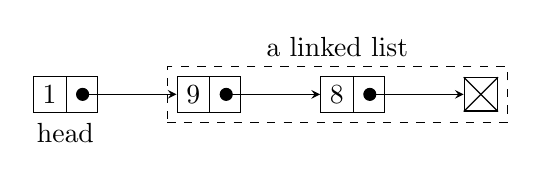
\begin{tikzpicture}[list/.style={rectangle split, rectangle split parts=2,
        draw, rectangle split horizontal}, >=stealth, start chain]
    
      \node[list,on chain] (A) {1};
      \node[list,on chain] (B) {9};
      \node[list,on chain] (C) {8};
      \node[on chain,draw,inner sep=6pt] (D) {};
      \draw (D.north east) -- (D.south west);
      \draw (D.north west) -- (D.south east);
      \draw[*->] let \p1 = (A.two), \p2 = (A.center) in (\x1,\y2) -- (B);
      \draw[*->] let \p1 = (B.two), \p2 = (B.center) in (\x1,\y2) -- (C);
      \draw[*->] let \p1 = (C.two), \p2 = (C.center) in (\x1,\y2) -- (D);
      \node[below=of A, yshift=1cm] (head){\alert{head}};
    
      \node[fit=(B)(C)(D), dashed, draw](remain) {};
    
      \node[above=of remain, yshift=-1cm]{\alert{a linked list}};
    \end{tikzpicture}

    \scalebox{.8}{  
        \begin{algorithm}[H]
            \setstretch{.9}
            \caption{reverseList(head)}
            $pre\gets null$ \\
            $cur\gets head$ \\
            \While{cur $\neq$ null} {
                $next\gets cur.next$ \\
                $cur.next\gets pre$ \\
                $pre\gets cur$ \\
                $cur\gets next$
            }
            \Return{pre}
            \end{algorithm}
    }

\end{frame}

\begin{frame}
\begin{itemize}
    \item \textbf{Case 1}: the list is empty.
    \item \textbf{Case 2}: the size is 1.
    \item \textbf{Case 3}: the size is greater than 1.
\end{itemize}

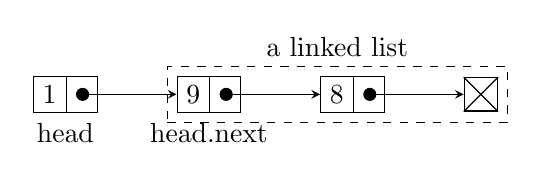
\begin{tikzpicture}[list/.style={rectangle split, rectangle split parts=2,
    draw, rectangle split horizontal}, >=stealth, start chain]

  \node[list,on chain] (A) {1};
  \node[list,on chain] (B) {9};
  \node[list,on chain] (C) {8};
  \node[on chain,draw,inner sep=6pt] (D) {};
  \draw (D.north east) -- (D.south west);
  \draw (D.north west) -- (D.south east);
  \draw[*->] let \p1 = (A.two), \p2 = (A.center) in (\x1,\y2) -- (B);
  \draw[*->] let \p1 = (B.two), \p2 = (B.center) in (\x1,\y2) -- (C);
  \draw[*->] let \p1 = (C.two), \p2 = (C.center) in (\x1,\y2) -- (D);
  \node[below=of A, yshift=1cm] (head){\alert{head}};

  \node[below=of B, yshift=1cm] {\alert{head.next}};

  \node[fit=(B)(C)(D), dashed, draw](remain) {};

  \node[above=of remain, yshift=-1cm]{\alert{a linked list}};
\end{tikzpicture}

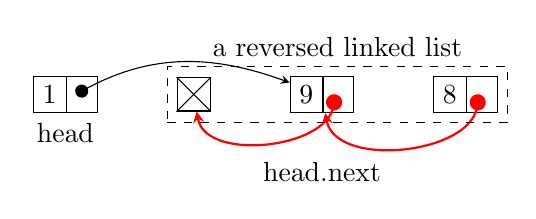
\begin{tikzpicture}[list/.style={rectangle split, rectangle split parts=2,
    draw, rectangle split horizontal}, >=stealth, start chain]

  \node[list,on chain] (A) {1};
  \node[on chain,draw,inner sep=6pt] (D) {};
  \draw (D.north east) -- (D.south west);
  \draw (D.north west) -- (D.south east);
  \node[list,on chain] (B) {9};
  \node[list,on chain] (C) {8};

  \draw[*->, red, thick] let \p1 = (C.two), \p2 = (C.center) in (\x1,\y2) to[out=-80,in=-80] (B);
  \draw[*->, red, thick] let \p1 = (B.two), \p2 = (B.center) in (\x1,\y2) to[out=-80,in=-80] (D);
  \draw[*->] let \p1 = (A.two), \p2 = (A.center) in (\x1,\y2) to[out=30,in=160] (B);
  \node[below=of A, yshift=1cm] (head){\alert{head}};

  \node[below=of B, yshift=.5cm] {\alert{head.next}};

  \node[fit=(B)(C)(D), dashed, draw](remain) {};

  \node[above=of remain, yshift=-1cm]{\alert{a reversed linked list}};
\end{tikzpicture}

\end{frame}

\begin{frame}

    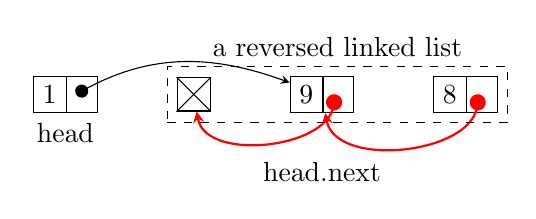
\begin{tikzpicture}[list/.style={rectangle split, rectangle split parts=2,
        draw, rectangle split horizontal}, >=stealth, start chain]
    
      \node[list,on chain] (A) {1};
      \node[on chain,draw,inner sep=6pt] (D) {};
      \draw (D.north east) -- (D.south west);
      \draw (D.north west) -- (D.south east);
      \node[list,on chain] (B) {9};
      \node[list,on chain] (C) {8};
    
      \draw[*->, red, thick] let \p1 = (C.two), \p2 = (C.center) in (\x1,\y2) to[out=-80,in=-80] (B);
      \draw[*->, red, thick] let \p1 = (B.two), \p2 = (B.center) in (\x1,\y2) to[out=-80,in=-80] (D);
      \draw[*->] let \p1 = (A.two), \p2 = (A.center) in (\x1,\y2) to[out=30,in=160] (B);
      \node[below=of A, yshift=1cm] (head){\alert{head}};
    
      \node[below=of B, yshift=.5cm] {\alert{head.next}};
    
      \node[fit=(B)(C)(D), dashed, draw](remain) {};
    
      \node[above=of remain, yshift=-1cm]{\alert{a reversed linked list}};
    \end{tikzpicture}
    
    \scalebox{.85}{  
        \begin{algorithm}[H]
            \caption{reverseList(head)}
            \If{head = null or head.next = null}{
                \Return{head}
            }
            $rest\gets reverseList(head.next)$ \\
            $head.next.next\gets head$ \\
            $head.next\gets null$\\
            \Return{rest}            
            \end{algorithm}
    }

\end{frame}

\begin{frame}
    \frametitle{2.4 Pros and Cons}
All recursions can be transformed into \textbf{iterative} algorithms. Generally, recursions make the code much cleaner, but they may result in several cons:

\begin{itemize}
    \item Slower.
    \item Larger memory overhead.
    \item Hard to analyze.
\end{itemize}

\end{frame}

\begin{frame}
\frametitle{Summary}

{\large \faIcon{lightbulb}} There are three important rules of thumb in developing recursive programs:

\begin{enumerate}
    \item The recursion has a \textbf{base case}.
    \item Recursive calls must address sub-problems that are \textbf{smaller} in some sense.
    \item Recursive calls should not address sub-problems that overlap.
\end{enumerate}
\end{frame}

\hanoi{3}

\begin{frame}[fragile]
    \frametitle{Towers of Hanoi}
To move $n$ disks from pole A to pole C, how many times of moving are required?

\begin{minted}[bgcolor=LightGray, baselinestretch=1]{python}
def move(n):
    assert n >= 0
    if n == 0 or n == 1:
        return n
    # move (n-1) disks from A to B, using C
    # move nth (largest) disk from A to C
    # move (n-1) disks from B to C, using A
    return 2 * move(n - 1) + 1
\end{minted}
\end{frame}

\begin{frame}
    \frametitle{Exercise 1: Towers of Hanoi}
    {\large \faIcon{code}} To develop a recursive algorithm to print the process of how those disks are moved.

\end{frame}

\begin{frame}[fragile]
    \frametitle{Exercise 2: Binary Search}
{\large \faIcon{code}} \textbf{Binary search}: return the index of a given \alert{key} in a sorted array.    

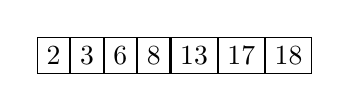
\begin{tikzpicture}
  
    \matrix[nodes=draw]
    {
      \node {2}; &
      \node {3}; &
      \node {6}; &
      \node {8}; &
      \node {13}; & 
      \node {17}; &
      \node {18}; \\
    };
  \end{tikzpicture}
  
  Compare the mid-item with the given \alert{key}:
  \begin{itemize}
    \item If the mid-item is larger, then search on the right side.
    \item If the mid-item is smaller, then search on the left side.
    \item Otherwise, bingo!
  \end{itemize}
\end{frame}

\begin{frame}[fragile]
The non-recursive version:

\begin{minted}[bgcolor=LightGray, baselinestretch=1]{python}
def search(a, target):
    high = len(a) - 1
    low = 0
    while high >= low:
        mid = low + (high - low) // 2
        if a[mid] == target:
            return mid
        elif a[mid] > target:
            high = mid - 1
        else:
            low = mid + 1
    return -1
\end{minted}
    

\end{frame}

\begin{frame}
    \frametitle{Homework 4}
\begin{itemize}
    \item Ex 9 or Ex 10, Chapter 3 (10 marks)
    \item Ex 13. (10 marks)
\end{itemize}
Note that pseudo-code is allowed.
\end{frame}
\end{document}